\chapter{Kotlin Multiplatform}\label{ch:kotlin-multiplatform}

The Kotlin Multiplatform (KMP) technology allows developers to share code across multiple platforms, such as Android and iOS for mobile applications, and/or JVM, JavaScript and Native for multiplatform overall.


\section{Project Structure}\label{sec:project-structure}

A Kotlin Multiplatform project is divided into three main categories of code:

\begin{itemize}
    \item \textbf{Common}: Code shared between all platforms (i.e., \textit{CommonMain, CommonTest});
    \item \textbf{Intermediate}: Code that can be shared on a subset of platforms (i.e., \textit{AppleMain, AppleTest});
    \item \textbf{Specific}: Code specific to a target platform (i.e., \texttt{\textit{<Platform>Main}}, \texttt{\textit{<Platform>Test}}).
\end{itemize}


An example of a Kotlin Multiplatform project architecture can be seen in Figure~\ref{fig:kmp-architecture}, but note that both \textit{Intermediate} and \textit{Specific} categories are optional.

\begin{figure}[!htb]
    \centering
    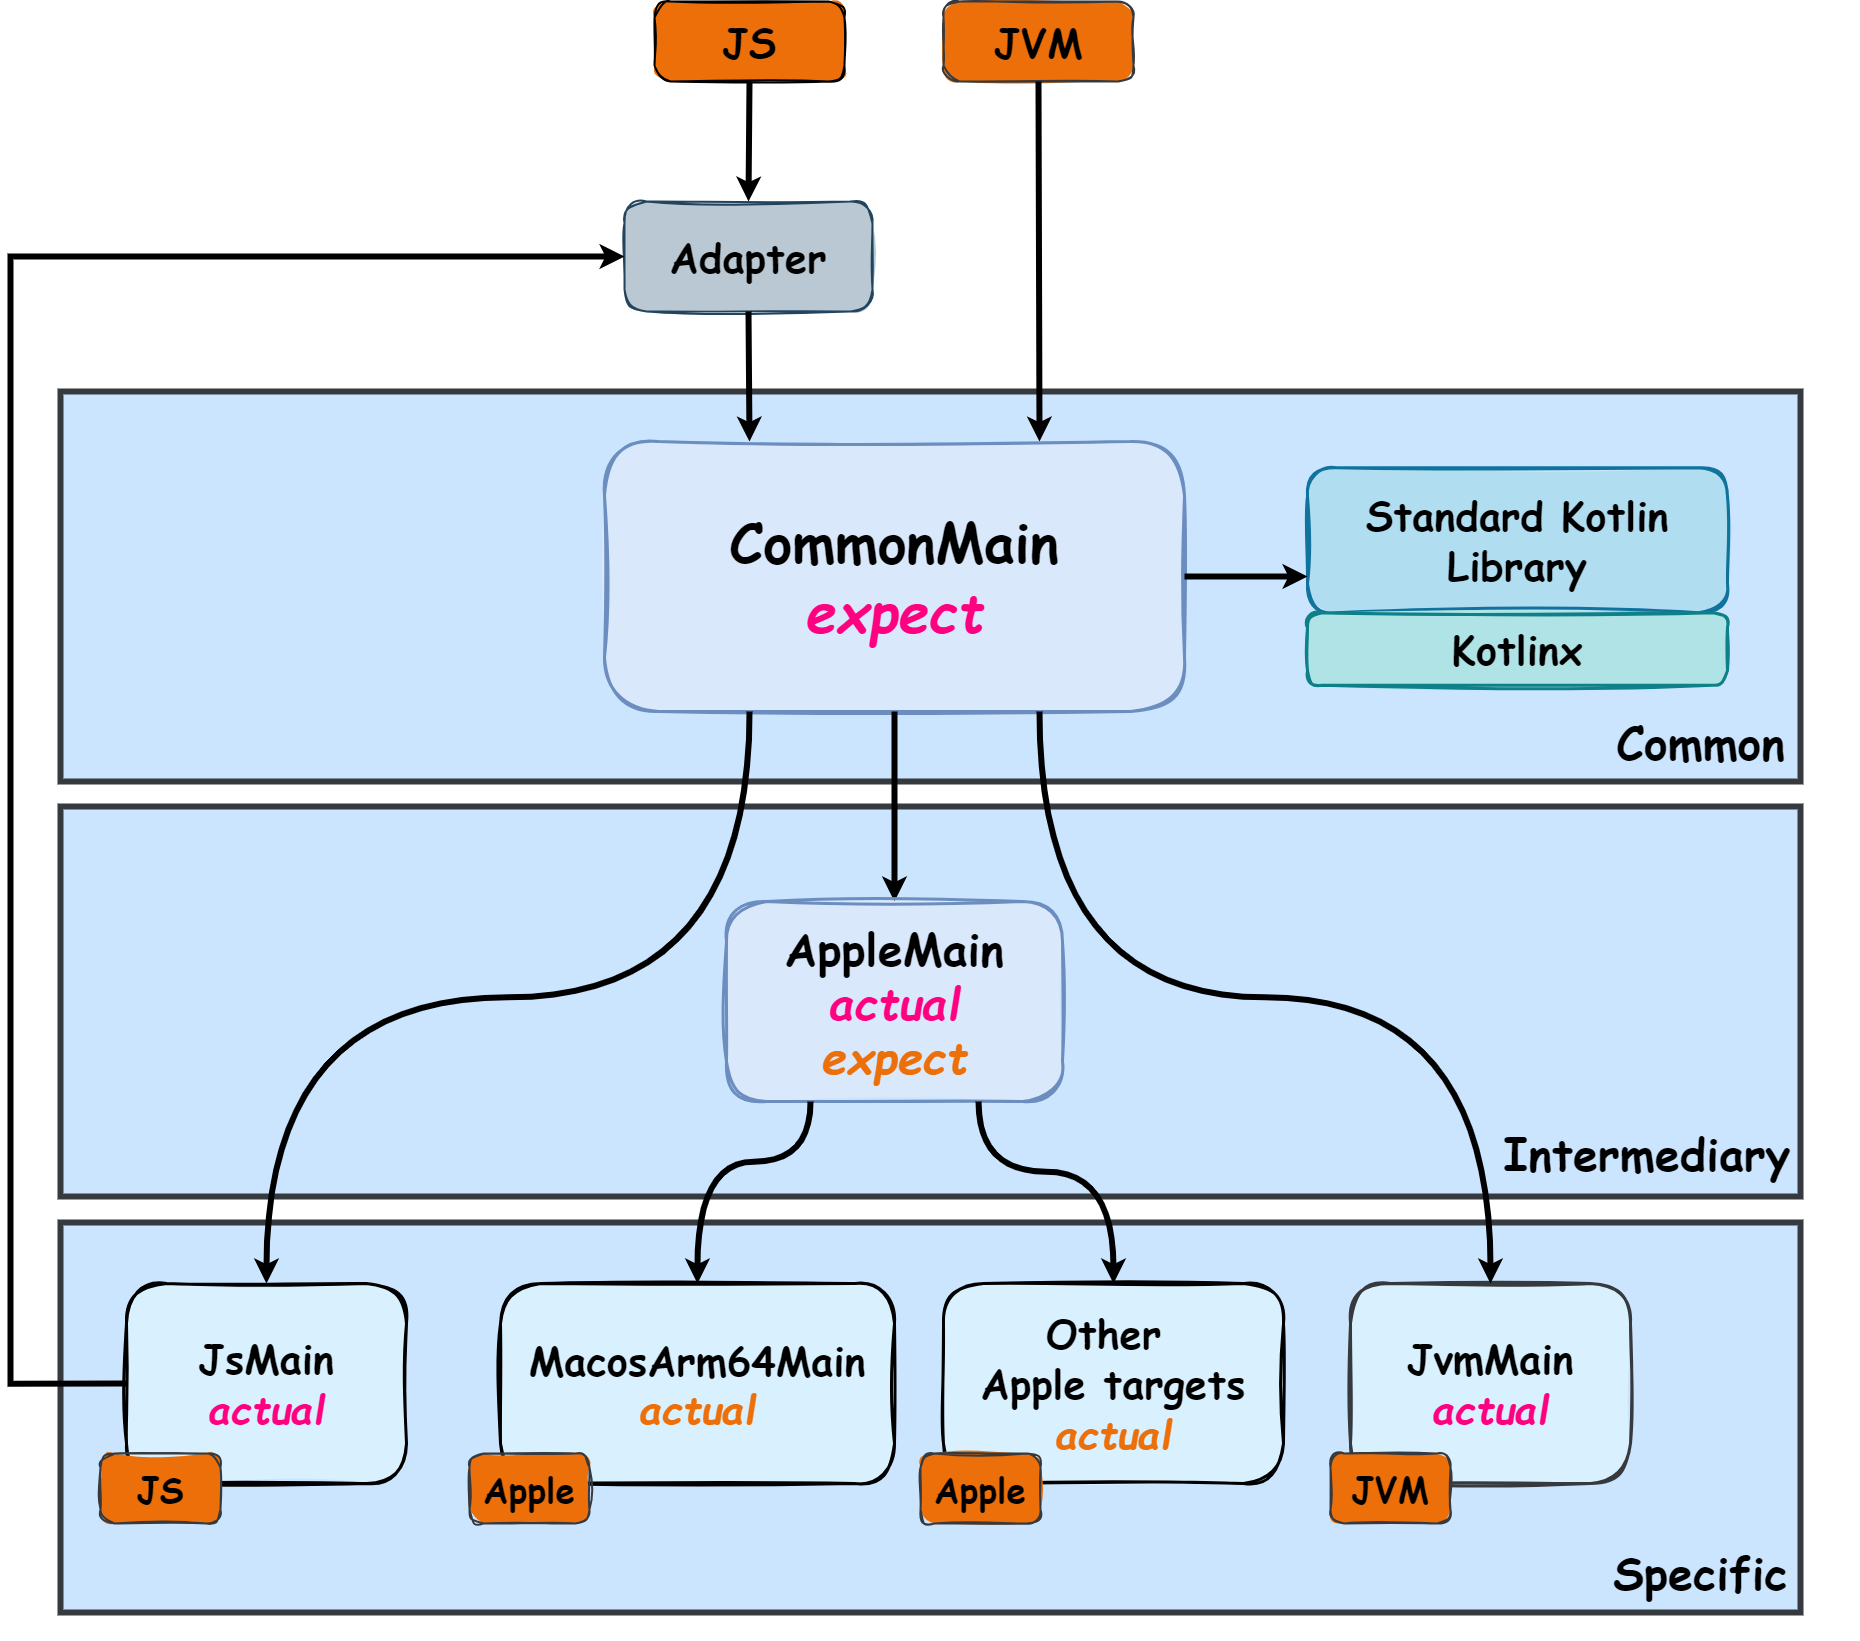
\includegraphics[width=0.9\textwidth]{../figures/02_kmp-architecture}
    \caption{Example of a \textit{KMP} project architecture.}
    \label{fig:kmp-architecture}
\end{figure}

\subsection{Template}\label{subsec:template}

Although it is possible to create a \textit{KMP} project from scratch, it is recommended to use a template that provides a standardized setup for developing Kotlin libraries and applications that target multiple platforms.
This project used the official template available from Kotlin's GitHub organization~\cite{kmp-github-template}.

\subsection{Gradle Tasks}\label{subsec:available-gradle-tasks}

Gradle is a build automation tool for multi-language software development.
Offers support for all phases of a build process including compilation, verification, dependency resolving, test execution, source code generation, packaging and publishing~\cite{gradle}.

In a Gradle build using Kotlin DSL (i.e., domain-specific language), the project's configuration is primarily defined in two key files:

\begin{itemize}
    \item \textbf{build.gradle.kts} - Defines the project's build configuration.
    In Kotlin Multiplatform projects, this file is used to define the project's targets, dependencies in the respective source sets, and additional configurations if needed;
    \item \textbf{settings.gradle.kts} - Defines the project's structure and modules it contains.
\end{itemize}

In Gradle, tasks are the smallest unit of work that can be executed and are used to perform specific actions.
The templated uses the Kotlin Multiplatform plugin which includes several pre-configured Gradle tasks to facilitate building, testing, and managing the project across multiple platforms configured as targets in the respective build gradle file.
Some of the key tasks are:

\begin{itemize}
    \item \textbf{Build}: Compiles and assembles the project;
    \item \textbf{AllTests}: Runs the test cases for all platforms.
    To run platform-specific tests, use the \texttt{<Platform>Test} task (e.g., \textit{jvmTest});
    \item \textbf{Check}: Performs various checks on the project, including running tests and performing additional operations (e.g., linting, code analysis);
    \item \textbf{Clean}: Deletes the build directory, allowing for a clean build (i.e., not using cached artifacts).
\end{itemize}

A Gradle project can be organized into multiple subprojects, each with its own build file, settings and tasks.

\subsection{GitHub Actions}\label{subsec:github-actions}

Provided by the template, the project utilizes GitHub Actions~\cite{github-actions} for continuous integration and continuous deployment (CI/CD)~\cite{redhat-cicd}.
The configurations for GitHub Actions are located in the \textit{.github/workflows} folder, and include the following workflows:

\begin{itemize}
    \item \textbf{gradle.yml} - Builds and tests the project using Gradle against some of the available platforms (e.g., Javascript was missing and was added manually).
    Runs on push and pull request events to the default branch;
    \item \textbf{deploy.yml} - deploys the library artifacts to a repository in Maven Central, following a pre-defined authentication configuration.
\end{itemize}

\subsection{Folder Structure}\label{subsec:folder-structure}

The project is organized into several folders, each serving a specific purpose.
Below is a brief description of each folder, with an emphasis on the \textit{src} folders:

\begin{itemize}
    \item \textbf{.github/}: Contains configurations for GitHub Actions, which are used to automate tasks;
    \item \textbf{gradle/}: Contains configuration files and scripts related to the Gradle build system.
    This folder typically includes:
    \begin{itemize}
        \item \textbf{wrapper/}: Contains the wrapper files and configurations, which standardizes a project on a given Gradle version for more reliable and robust builds~\cite{gradle-wrapper};
        \item \textbf{libs.versions.toml}: Defines the versions of the libraries and plugins used in the project, as dependencies, in a centralized manner (regularly known as version catalog).
    \end{itemize}
    \item \textbf{convention-plugins/}: Encapsulates and reuses common build logic across multiple Gradle projects or modules (e.g., for publishing, testing, etc.);
    \item \textbf{library/}: Contains the source code for the library and the build configuration file.
    \begin{itemize}
        \item \textbf{src/}: Contains the source code for the library, divided into multiple submodules based on the target platforms:
        \begin{itemize}
            \item \textbf{commonMain/}: Contains the common code shared across all platforms;
            \item \textbf{jvmMain/}: Contains the source code specific to the JVM platform;
            \item \textbf{jsMain/}: Contains the source code specific to the JavaScript platform;
            \item \textbf{iosMain/}: Contains the source code specific to the iOS platform;
            \item \textbf{androidMain/}: Contains the source code specific to the Android platform;
            \item And all of these module counterparts for the test code (e.g., \textit{commonTest, jvmTest, jsTest, etc}).
        \end{itemize}
        \item \textbf{build.gradle.kts}: Defines the targets, dependencies, and additional configurations for the library;
    \end{itemize}
    \item \textbf{build.gradle.kts}: The main build configuration file for the project, where the project's modules common dependencies are defined;
    \item \textbf{settings.gradle.kts}: Configures the Gradle build settings for the project, including the root project name and module inclusion.
\end{itemize}

Based on the described template's project structure, the following project structure was adopted for developing a Kotlin Multiplatform library:

\begin{itemize}
    \item \textbf{\texttt{<}kmp\_package\_name\texttt{>}}: name of the Kotlin Multiplatform library in root directory;
    \begin{itemize}
        \item \textbf{apps}: defines the modules that will consume the \textitKMP library (e.g.,\textttt{js-app}, \texttt{android-app});
        \item \textbf{lib/shared}: defines the library's code to be shared by the consuming modules;
        \begin{itemize}
            \item \textbf{src} defines the target submodules of the library including their test counterparts (i.e., \texttt{<Platform>Main}, \texttt{<Platform>Test}).
            \item \textbf{build.gradle.kts}: defines the library's dependencies, targets, and additional configurations.
        \end{itemize}
    \end{itemize}
\end{itemize}


\section{Platform-Dependent Code}\label{sec:platform-dependent-code}

As code sharing across platforms is the primary objective of \textit{KMP}, the code should be written as platform-independently as possible (i.e., aggregating as much code as possible in the hierarchically higher categories).
However, it is sometimes necessary to create specific code for a given platform, regularly referred to as \textit{target}, in the following situations:

\begin{itemize}
    \item Access to API's specific to the \textit{target} is required (e.g., \textit{Java's File API});
    \item The libraries available in the common category (i.e., \textit{Standard Kotlin Library}, libraries from \textit{Kotlinx}) do not cover the desired functionalities and third-party libraries either don't support it or dependency reduction is desired;
    \item A given \textit{target} does not directly support \textit{KMP} (e.g., \textit{Node.js)}, and so it is necessary to create an \textit{adapter}.
    This adapter allows communication with the common category code, in \textit{Kotlin}, from the native code of the \textit{target}, which can be defined in the \textit{Intermediate} or \textit{Specific} category.
\end{itemize}

To create specific code for a \textit{target}, the mechanism \textit{expect/actual}~\cite{kmp-expect-actual} is used.
This mechanism allows defining the code to be implemented in an abstracted way and its implementation, respectively.


\section{Supported Targets}\label{sec:supported-targets}

The project supports the following targets:

\begin{itemize}
    \item \textbf{JVM}: Allows running the code on the Java Virtual Machine;
    \item \textbf{JavaScript}: Allows running the code in a browser or Node.js environment;
    \item \textbf{Android}: Allows running the code on Android devices.
    \item \textbf{Native}: Allows running the code on platforms that support Kotlin/Native, excluding macOS and iOS, because the lack of access to the necessary hardware for testing.
\end{itemize}

\section{Running Tests}\label{sec:running-tests}
TODO


\section{Other Aspects}\label{sec:other-aspects}
TODO: What was done to have concurrency, logging, CI integration, etc
